% ==============================================================================
% Section 1.9: Case Study — Neutrino
% ==============================================================================

\section{Case Study: Neutrino}
\label{sec:case_neutrino}

\subsection{The Edge Mode and Ledger Partner}

% --- AT-A-GLANCE BOX (KB-CANON-002) ---
\begin{edcAtAGlance}{Neutrino Properties}
  \edcBaseline{
    Mass: Very small, $m_\nu \lesssim 1$ eV (from oscillation data)\\
    Chirality: Only left-handed neutrinos couple to weak interactions\\
    Interactions: Extremely weak (mean free paths of astronomical scale)\\
    Role: ``Missing'' particle in all weak decays (carries energy \& lepton number)
  }
  \edcEDCView{
    Neutrino = edge mode at bulk--brane interface (not interior mode)\\
    Weak coupling arises from suppressed wavefunction overlap, not small $g$\\
    Chirality selection encoded in boundary conditions ($\mathcal{P}_{\mathrm{chir}}$)\\
    Ledger closure partner: required to balance energy/quantum numbers
  }
  \edcKeyInsight{
    Neutrinos are not ``add-ons'' but essential partners. Their edge-mode localization
    explains both their weak interactions (small overlap) and their role in every
    weak decay (ledger closure). The V$-$A structure may be a boundary phenomenon.
  }
  \edcFalsifiable{
    \textbullet\ If right-handed neutrinos couple at comparable strength to left-handed\\
    \textbullet\ If neutrino masses are much larger than sub-eV\\
    \textbullet\ If neutrino interactions are stronger than geometric overlap predicts
  }
\end{edcAtAGlance}

\medskip

% ==============================================================================
\subsubsection{Motivation: The Neutrino Problem}
% ==============================================================================

In the EDC Weak Program, every decay process closes a \emph{ledger}: energy,
momentum, charge, and quantum numbers must balance across bulk, brane, and
3D outputs. The neutrino plays a unique role: it carries away ``missing''
quantities without being detected as a charged particle.

The Standard Model treats neutrinos as fundamental fermions with extremely
small cross-sections. EDC reinterprets this:

\begin{tcolorbox}[edcCornerstone, title={Core Reinterpretation \tagP{}}]
The neutrino is not ``weakly interacting because it escapes into the bulk.''
Instead, it is a \textbf{boundary/edge mode}---an excitation localized at the
bulk-brane interface whose coupling to observer-facing states is
\textbf{suppressed by boundary conditions}.
\end{tcolorbox}

This reinterpretation has advantages:
\begin{enumerate}[nosep]
  \item No need for ``leakage into 5D'' (which would violate 4D energy
        conservation from the observer perspective)
  \item Explains helicity/chirality structure via boundary conditions
  \item Provides a natural ledger-closure mechanism
\end{enumerate}

\begin{tcolorbox}[edcGuardrail, title={Scope Guardrail}]
\begin{itemize}[nosep]
  \item We do \textbf{not} derive neutrino masses (mass origin (open))
  \item We do \textbf{not} address neutrino oscillations in this document
        ((open))
  \item We \textbf{do} explain the neutrino's structural role in ledger
        closure and why it appears ``invisible'' to charged-current
        interactions after emission
\end{itemize}
\end{tcolorbox}

% ==============================================================================
\subsubsection{The Interfacial Zone}
% ==============================================================================

Recall from Section~\ref{sec:case_electron} that the thick brane has three
conceptual layers. The neutrino resides in a fourth structural element: the
\emph{interface} between bulk and brane.

\begin{definition}[Interfacial Zone {\normalfont}]
\label{def:interfacial_zone}
The \textbf{interfacial zone} is the transitional region between the bulk
(5D) and the internal brane layer. It is characterized by:
\begin{enumerate}[nosep]
  \item \textbf{Partial localization:} modes here are neither fully bulk nor
        fully brane-bound
  \item \textbf{Boundary-condition sensitivity:} excitations must satisfy
        matching conditions between bulk and brane
  \item \textbf{Suppressed observer coupling:} direct interaction with
        observer-facing layer is exponentially suppressed
\end{enumerate}
\end{definition}

\paragraph{Neutrino localization diagram.}
\begin{center}
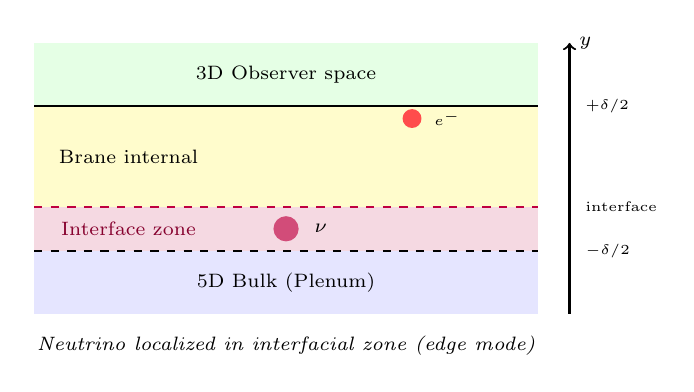
\begin{tikzpicture}[scale=0.8]
  % Bulk region
  \fill[blue!10] (-4,-2.5) rectangle (4,-1.5);
  \node[font=\scriptsize] at (0,-2) {5D Bulk (Plenum)};

  % Interfacial zone (neutrino region)
  \fill[purple!15] (-4,-1.5) rectangle (4,-0.8);
  \node[font=\scriptsize, purple!70!black] at (-2.5,-1.15) {Interface zone};

  % Brane internal layer
  \fill[yellow!20] (-4,-0.8) rectangle (4,0.8);
  \node[font=\scriptsize] at (-2.5,0) {Brane internal};

  % Observer region
  \fill[green!10] (-4,0.8) rectangle (4,1.8);
  \node[font=\scriptsize] at (0,1.3) {3D Observer space};

  % Neutrino defect (in interface)
  \fill[purple!70] (0,-1.15) circle (0.2);
  \node[font=\scriptsize\bfseries, right] at (0.3,-1.15) {$\nu$};

  % Electron for comparison (on observer side)
  \fill[red!70] (2,0.6) circle (0.15);
  \node[font=\tiny, right] at (2.2,0.6) {$e^-$};

  % Boundaries
  \draw[thick, dashed] (-4,-1.5) -- (4,-1.5);
  \draw[thick, dashed, purple] (-4,-0.8) -- (4,-0.8);
  \draw[thick] (-4,0.8) -- (4,0.8);

  % y-axis
  \draw[->, thick] (4.5,-2.5) -- (4.5,1.8);
  \node[font=\scriptsize, right] at (4.5,1.8) {$y$};
  \node[font=\tiny, right] at (4.6,0.8) {$+\delta/2$};
  \node[font=\tiny, right] at (4.6,-0.8) {interface};
  \node[font=\tiny, right] at (4.6,-1.5) {$-\delta/2$};

  % Caption annotation
  \node[font=\scriptsize\itshape, align=center] at (0,-3)
    {Neutrino localized in interfacial zone (edge mode)};
\end{tikzpicture}
\end{center}

% ==============================================================================
\subsubsection{Neutrino Ontology: Edge Mode Definition}
% ==============================================================================

\begin{postulate}[Neutrino as Edge Mode {\normalfont \tagP{}/}]
\label{post:neutrino_edge}
The neutrino is an \textbf{edge mode}---a boundary excitation that:
\begin{enumerate}[nosep]
  \item Carries conserved quantum numbers (lepton number, spin, helicity)
  \item Is localized at the bulk-brane interface (not inside bulk, not on
        observer-facing layer)
  \item Has \textbf{suppressed leakage} into both bulk and observer-facing
        regions due to boundary conditions
  \item Appears as three flavors ($\nu_e$, $\nu_\mu$, $\nu_\tau$) corresponding
        to the charged lepton sector
\end{enumerate}
\end{postulate}

\edcMechanismNote{Bulk-brane energy exchange creates interface excitation}%
                 {Boundary conditions localize mode at interface; chirality filter selects helicity}%
                 {Neutrino carries ledger balance (spin, momentum, lepton number) away from decay vertex}

\textbf{Key distinction from ``bulk escape.''}
The neutrino does not ``escape into the 5th dimension.'' It remains
interface-localized. Its weak interaction with 3D matter arises from
\emph{suppressed coupling} across the interface, not from being ``elsewhere.''

\begin{tcolorbox}[edcGuardrail, title={Language Precision}]
\textbf{Avoid:} ``The neutrino cannot interact because it escapes into the
bulk.''

\textbf{Use:} ``The neutrino's coupling to observer-facing states is
\textbf{suppressed by boundary conditions} at the interface.'' \tagP{}

This avoids implying energy loss to extra dimensions (which would violate
observed 4D conservation).
\end{tcolorbox}

% ==============================================================================
\subsubsection{PDG Baselines}
% ==============================================================================

\begin{table}[ht]
\centering
\caption{Neutrino baseline properties (PDG 2024) \tagBL{}}
\label{tab:neutrino_baselines}
\begin{tabular}{lll}
\toprule
\textbf{Property} & \textbf{Value} & \textbf{EDC Interpretation} \\
\midrule
Mass upper bound & $m_{\nu_e} < 0.8$ eV (direct) & Edge-mode energy (open) \\
$\Delta m^2_{21}$ & $7.53 \times 10^{-5}$ eV$^2$ & Mode splittings (open) \\
$\Delta m^2_{31}$ & $2.453 \times 10^{-3}$ eV$^2$ & Mode splittings (open) \\
Dirac/Majorana & Unknown & Nature of edge mode (open) \\
Chirality & Left-handed only & BC selection \tagP{} \\
\bottomrule
\end{tabular}
\end{table}

% ==============================================================================
\subsubsection{Why Neutrinos Interact Weakly}
% ==============================================================================

In the Standard Model, neutrinos interact only via $W^\pm$ and $Z^0$ exchange,
which is suppressed by the large gauge boson masses \tagBL{}.

In EDC, the interpretation is geometric \tagP{}/\tagDc{}:

\begin{tcolorbox}[edcCornerstone, title={Neutrino Weak Coupling: Geometric Origin \tagP{}}]
\textbf{Claim}: The neutrino's edge-mode localization means its wavefunction
has suppressed overlap with bulk modes and brane-interior modes.

\textbf{Consequence}: The effective coupling of neutrinos to other particles
is controlled by overlap integrals:
\begin{equation}
g_{\nu,\mathrm{eff}} \propto \int_{\text{brane}} \psi_\nu^*(\xi) \cdot
\psi_{\text{other}}(\xi) \cdot \phi_{\text{mediator}}(\xi) \, d\xi,
\label{eq:nu_effective_coupling}
\end{equation}
which is suppressed because $\psi_\nu(\xi)$ is localized at the edge while
other particles are localized in the interior.
\end{tcolorbox}

This provides a geometric origin for ``weak interactions'': they are weak
because of suppressed overlap, not because of a small fundamental coupling.

The suppression mechanism in detail:
\begin{enumerate}[nosep]
  \item Neutrino is interface-localized (edge mode)
  \item Observer-facing layer is separated by internal brane layer
  \item Coupling across layers is exponentially suppressed by wavefunction
        overlap \tagP{}
  \item Result: neutrino appears ``invisible'' after emission
\end{enumerate}

% ==============================================================================
\subsubsection{Ledger Role: What the Neutrino Carries}
% ==============================================================================

In every weak decay, the neutrino (or antineutrino) closes the conservation
ledger:

\begin{table}[ht]
\centering
\caption{Neutrino ledger contributions in representative decays \tagBL{}}
\label{tab:neutrino_ledger}
\begin{tabular}{lcccc}
\toprule
\textbf{Decay} & \textbf{Energy} & \textbf{Momentum} & \textbf{Spin} & \textbf{Lepton \#} \\
\midrule
$n \to p + e^- + \bar\nu_e$ & $E_\nu$ & $\vec{p}_\nu$ & $+1/2$ (RH) & $-1$ \\
$\mu^- \to e^- + \bar\nu_e + \nu_\mu$ & $E_{\nu_\mu}, E_{\bar\nu_e}$ & balanced & mixed & $0$ (net) \\
$\pi^- \to \mu^- + \bar\nu_\mu$ & $E_{\bar\nu_\mu}$ & $\vec{p}_{\bar\nu}$ & $+1/2$ (RH) & $-1$ \\
$\tau^- \to e^- + \bar\nu_e + \nu_\tau$ & $E_{\nu_\tau}, E_{\bar\nu_e}$ & balanced & mixed & $0$ (net) \\
\bottomrule
\end{tabular}
\end{table}

\textbf{Pattern.}
The neutrino is the ``minimal-energy neutral partner'' required to close
the ledger while conserving lepton number \tagDc{}. Its appearance is not
accidental but structural.

% ==============================================================================
\subsubsection{Chirality Selection: The Chiral Filter}
% ==============================================================================

A striking feature of neutrinos is that only left-handed neutrinos (and
right-handed antineutrinos) couple to weak interactions \tagBL{}.

In EDC, this is encoded in $\mathcal{P}_{\mathrm{chir}}$ as a boundary effect
\tagP{}:

\begin{definition}[Chirality Filter {\normalfont \tagP{}/\tagDc{}}]
\label{def:neutrino_chiral}
The brane boundary conditions select:
\begin{itemize}[nosep]
  \item \textbf{Left-handed} charged leptons ($e^-_L$, $\mu^-_L$, $\tau^-_L$)
  \item \textbf{Right-handed} antineutrinos ($\bar\nu_R$)
  \item \textbf{Left-handed} neutrinos ($\nu_L$)
\end{itemize}
In the massless limit, helicity equals chirality. For massive particles,
the boundary condition selects chirality; helicity follows approximately.
\end{definition}

\paragraph{Chiral projection operator.}
We define $\mathcal{P}_{\mathrm{chir}}$ that encodes the chirality selection:

\begin{definition}[Chiral Projection Operator {\normalfont \tagP{}/}]
\label{def:pchir_neutrino}
The operator $\mathcal{P}_{\mathrm{chir}}$ acts on fermion modes at the brane
boundary:
\begin{align}
  \mathcal{P}_{\mathrm{chir}} \psi_{\ell^-} &= P_L\psi_{\ell^-} = \tfrac{1}{2}(1-\gamma_5)\psi_{\ell^-}
    \quad \text{(left-handed charged lepton)} \\
  \mathcal{P}_{\mathrm{chir}} \psi_{\bar\nu} &= P_R\psi_{\bar\nu} = \tfrac{1}{2}(1+\gamma_5)\psi_{\bar\nu}
    \quad \text{(right-handed antineutrino)}
\end{align}
where $L/R$ refer to chirality eigenstates.
\end{definition}

\textbf{V$-$A consistency.}
The operator $\mathcal{P}_{\mathrm{chir}}$ is postulated \tagP{} to arise from
the boundary conditions at the bulk-brane interface. It produces V$-$A
structure as an \emph{output}, not an input assumption:
\begin{equation}
  \mathcal{J}^\mu_{\mathrm{weak}} \propto \bar\psi_{\ell,L} \gamma^\mu \psi_{\nu,L}
  = \bar\psi_\ell \gamma^\mu (1 - \gamma^5) \psi_\nu / 2
\label{eq:nu_VA_current}
\end{equation}
which is the standard V$-$A current \tagBL{}.

\paragraph{Chirality filter diagram.}
\begin{center}
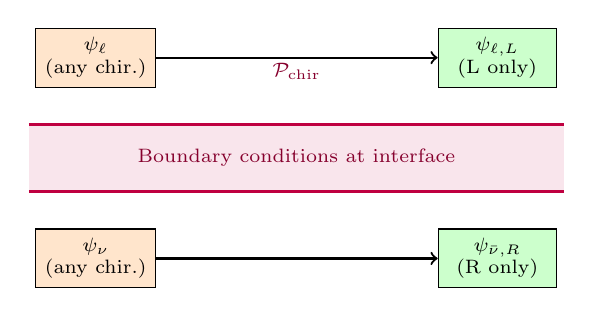
\begin{tikzpicture}[scale=0.85]
  % Interface zone
  \fill[purple!10] (-4,-0.5) rectangle (4,0.5);
  \draw[thick, purple] (-4,0.5) -- (4,0.5);
  \draw[thick, purple] (-4,-0.5) -- (4,-0.5);
  \node[font=\scriptsize, purple!70!black] at (0,0) {Boundary conditions at interface};

  % Left side: inputs
  \node[rectangle, draw, fill=orange!20, font=\scriptsize, minimum width=1.5cm, align=center] (inL) at (-3,1.5)
    {$\psi_{\ell}$\\(any chir.)};
  \node[rectangle, draw, fill=orange!20, font=\scriptsize, minimum width=1.5cm, align=center] (inN) at (-3,-1.5)
    {$\psi_{\nu}$\\(any chir.)};

  % Right side: outputs
  \node[rectangle, draw, fill=green!20, font=\scriptsize, minimum width=1.5cm, align=center] (outL) at (3,1.5)
    {$\psi_{\ell,L}$\\(L only)};
  \node[rectangle, draw, fill=green!20, font=\scriptsize, minimum width=1.5cm, align=center] (outN) at (3,-1.5)
    {$\psi_{\bar\nu,R}$\\(R only)};

  % Simplified arrows: inputs to filter, filter to outputs
  \draw[->, thick] (inL) -- (outL);
  \draw[->, thick] (inN) -- (outN);

  % Filter annotation
  \node[font=\scriptsize\bfseries, purple!70!black] at (0,1.3) {$\mathcal{P}_{\mathrm{chir}}$};

\end{tikzpicture}
\end{center}

\paragraph{Physical picture.}
The bulk-brane interface imposes boundary conditions on spinor fields. These
boundary conditions select a particular chirality for the edge mode. The
``other'' chirality (right-handed neutrino) either:
\begin{enumerate}[nosep]
  \item Does not satisfy the boundary conditions (is projected out), or
  \item Has a different localization (propagates into the bulk) and thus
        does not appear as a 3D edge mode.
\end{enumerate}

% ==============================================================================
\subsubsection{Neutrino Mass: An Edge-Mode Energy}
% ==============================================================================

If neutrinos are edge modes, their mass should be related to the edge-mode
energy in the thick-brane geometry \tagP{}.

\paragraph{Expected scaling.}
Edge modes typically have energies suppressed relative to interior modes.
This is consistent with $m_\nu \ll m_e$:
\begin{equation}
\frac{m_\nu}{m_e} \sim e^{-\text{(separation parameter)}} \ll 1.
\label{eq:nu_mass_scaling}
\end{equation}

\paragraph{Open problem.}
Deriving the neutrino mass scale (sub-eV) from the edge-mode spectrum requires
solving the mode equation with appropriate boundary conditions (open).

% ==============================================================================
\subsubsection{Role as Ledger Closure Partner}
% ==============================================================================

In every weak decay, neutrinos appear as the ``missing'' particles that carry
away energy and lepton number:
\begin{itemize}[nosep]
  \item Neutron: $n \to p + e^- + \bar\nu_e$ ($\bar\nu_e$ carries $L_e = -1$)
  \item Muon: $\mu^- \to e^- + \bar\nu_e + \nu_\mu$ (two neutrinos share energy)
  \item Pion: $\pi^+ \to \mu^+ + \nu_\mu$ ($\nu_\mu$ carries $L_\mu = +1$)
  \item Tau: $\tau^- \to e^- + \bar\nu_e + \nu_\tau$ (two neutrinos share energy)
\end{itemize}

This pattern is not accidental. The neutrino is the ``minimal-energy neutral
partner'' required to close the ledger while conserving lepton number \tagDc{}.

% ==============================================================================
\subsubsection{Generative Closure Principle (Complete)}
\label{sec:generative_closure_complete}
% ==============================================================================

Together with the electron, neutrinos complete the \emph{Generative Closure
Principle}:

\begin{tcolorbox}[edcConcept, title={Generative Closure Principle (Complete) \tagP{}/\tagDc{}}]
A stable universe-like output sector requires:
\begin{enumerate}[nosep]
  \item A \textbf{lightest charged defect} (electron) that serves as the
        endpoint for all charged cascades
  \item \textbf{Excited states} of that sector (muon, tau) to allow cascades
        and composites
  \item \textbf{Ledger closure via neutral edge modes} (neutrinos) so that
        energy can be transferred, redistributed, and released without
        violating conservation
  \item A \textbf{massless neutral mode} (photon) that mediates long-range
        interactions
\end{enumerate}

\textbf{Guardrail}: This does not claim a full SM derivation. It asserts a
mechanism-level closure requirement and leaves explicit constructive
derivations as (open).
\end{tcolorbox}

% ==============================================================================
\subsubsection{Connection to Weak Companions}
% ==============================================================================

The neutrino edge-mode picture is consistent with all Weak Program companions:

\begin{itemize}[nosep]
  \item \textbf{Companion N} (Neutron, Section~\ref{sec:case_neutron}):
        $\bar\nu_e$ carries away lepton number $-1$, momentum, and part of
        $Q_\beta$
  \item \textbf{Companion M} (Muon, Section~\ref{sec:case_muon}): two neutrinos
        ($\nu_\mu$, $\bar\nu_e$) share the energy spectrum; interference
        requires both to be edge modes
  \item \textbf{Companion T} (Tau, Section~\ref{sec:case_tau}): multiple
        neutrino channels with flavor-matched partners
  \item \textbf{Companion P} (Pion, Section~\ref{sec:case_pion}): $\bar\nu_\mu$
        enables helicity suppression by carrying opposite helicity to $\mu^-$
  \item \textbf{Companion L} (Electron, Section~\ref{sec:case_electron}):
        neutrino completes the ledger, allowing electron selection
\end{itemize}

% ==============================================================================
\subsubsection{Process Diagram: Neutrino in Weak Decay}
% ==============================================================================

\begin{center}
\begin{tikzpicture}[scale=0.85]

% Bulk region
\fill[gray!15] (-4,2) rectangle (4,3);
\node[font=\small] at (0,2.5) {Bulk};

% Brane layer
\fill[blue!10] (-4,0.5) rectangle (4,2);
\draw[thick, blue!50] (-4,2) -- (4,2);
\draw[thick, blue!50] (-4,0.5) -- (4,0.5);
\node[font=\small, blue!60!black] at (0,1.25) {Brane Interior};

% Edge region (where neutrino lives)
\fill[purple!15] (-4,1.7) rectangle (4,2);
\draw[thick, purple!50, dashed] (-4,1.7) -- (4,1.7);
\node[font=\scriptsize, purple!60!black] at (3,1.85) {Edge};

% Observer region
\fill[green!10] (-4,-0.2) rectangle (4,0.5);
\node[font=\small, green!50!black] at (0,0.15) {Observer (3D)};

% Neutrino wavefunction
\draw[thick, purple] plot[smooth, domain=-3:3] (\x, {1.85 + 0.1*exp(-\x*\x)});
\node[font=\scriptsize, purple] at (-2.5,2.2) {$\psi_\nu(y)$};

% Electron wavefunction (for comparison)
\draw[thick, green!60!black] plot[smooth, domain=-3:3]
  (\x, {1.25 + 0.3*exp(-(\x-0.5)*(\x-0.5)/2)});
\node[font=\scriptsize, green!50!black] at (2,1.5) {$\psi_e(y)$};

% Overlap region annotation
\draw[{Stealth}-{Stealth}, thick, red!50] (-1,1.7) -- (-1,1.4);
\node[font=\tiny, red!50!black, right] at (-0.9,1.55) {small overlap};

% Ledger annotation
\node[rectangle, draw=gray, rounded corners=2pt, fill=gray!5,
      font=\tiny, align=center, text width=2.5cm] at (-2.5,-0.8)
  {Neutrinos close the\\ledger in all weak decays};

\end{tikzpicture}
\end{center}

% ==============================================================================
\subsubsection{Falsifiability Hooks}
% ==============================================================================

\begin{tcolorbox}[edcWarning, title={Falsifiability Handles}]
The neutrino-as-edge-mode hypothesis would be \textbf{challenged} if:
\begin{enumerate}[nosep]
  \item \textbf{Wrong-sign helicity:} Neutrino detected with wrong-sign
        helicity at appreciable rate (would require BC modification)
  \item \textbf{Ledger closure fails:} Missing energy not accountable to
        neutrino spectrum
  \item \textbf{Bulk-like propagation:} Neutrino showed different dispersion
        relation at high energy
  \item \textbf{Sterile mixing:} Sterile neutrino mixing violated interface
        localization picture
  \item \textbf{Right-handed $W$:} Discovery of right-handed $W$ bosons with
        SM-like coupling
  \item \textbf{V$+$A component:} Charged-current interactions showed V$+$A
        component at any scale
  \item \textbf{Lepton number violation:} Decay observed that violates lepton
        number without neutrinos
\end{enumerate}
Current experimental data are consistent with EDC edge-mode predictions
\tagBL{}.
\end{tcolorbox}

% ==============================================================================
\subsubsection{Open Questions}
% ==============================================================================

\begin{table}[ht]
\centering
\caption{Open questions and observable handles for neutrino physics}
\label{tab:neutrino_open}
\begin{tabular}{p{5.5cm}p{6cm}}
\toprule
\textbf{Open Question} & \textbf{Observable Handle} \\
\midrule
Origin of neutrino masses & Oscillation parameters, cosmological bounds
(open) \\
Why three flavors & Mode spectrum from interface geometry (open) \\
Dirac vs Majorana nature & Neutrinoless double-beta decay \tagBL{} \\
Sterile neutrino coupling & Short-baseline oscillation anomalies \tagBL{} \\
Explicit BC calculation & Mathematical formalization (open) \\
Mass hierarchy origin & Normal vs inverted ordering \tagBL{}/(open) \\
\bottomrule
\end{tabular}
\end{table}

% ==============================================================================
\subsubsection{Canonical Glossary}
% ==============================================================================

\begin{tcolorbox}[edcCanonical, title={Canonical Definitions: Neutrino Physics}]
\begin{description}[style=nextline, leftmargin=1.5em, font=\normalfont\itshape]
  \item[Edge mode]
    A boundary excitation localized at the bulk-brane interface, neither fully
    bulk nor fully brane-bound. \tagP{}/

  \item[Interfacial zone]
    The transitional region between bulk and brane where edge modes (neutrinos)
    are localized.

  \item[Suppressed leakage]
    The mechanism by which neutrino coupling to observer-facing states is
    exponentially suppressed by boundary conditions, rather than ``bulk
    escape.'' \tagP{}

  \item[Chirality filter ($\mathcal{P}_{\mathrm{chir}}$)]
    The boundary-condition operator that selects left-handed charged leptons
    and right-handed antineutrinos. \tagP{}/

  \item[V$-$A structure]
    The vector-minus-axial form of weak currents, which emerges as an
    \emph{output} of the chirality filter in EDC. \tagDc{}

  \item[Ledger closure partner]
    The neutrino's role as the minimal-energy neutral mode required to balance
    energy, momentum, and lepton number in weak decays. \tagDc{}

  \item[Generative closure]
    The principle that a stable output sector requires both charged endpoints
    (electron) and neutral ledger partners (neutrinos). \tagP{}
\end{description}
\end{tcolorbox}

